\RequirePackage[OT1]{fontenc}
\documentclass[conference]{IEEEtran}
\usepackage{amsmath,amssymb,graphicx,booktabs,array,tabularx,xurl,placeins,cite}
\usepackage[hidelinks]{hyperref}
\usepackage{xeCJK}
\setmainfont[BoldFont=texgyretermes-bold.otf,ItalicFont=texgyretermes-italic.otf,BoldItalicFont=texgyretermes-bolditalic.otf]{texgyretermes-regular.otf}
\setCJKmainfont[BoldFont=FandolSong-Bold.otf,ItalicFont=FandolKai-Regular.otf]{FandolSong-Regular.otf}
\setCJKsansfont[BoldFont=FandolHei-Bold.otf]{FandolHei-Regular.otf}
\title{MarsPro：缺失标签感知的多胁迫关联蛋白预测与领域适配逆折叠}
\author{}
\begin{document}
\maketitle


\begin{abstract}
跨胁迫条件整合蛋白资源会产生计算蛋白质组学中的缺失标签问题：一条序列在某一条件下有标注时，其他条件通常是未观测状态，而不是负例。本文提出\textbf{MarsPro}，由40,000条序列的MarsDataset、六输出序列预测器MarsClass和领域适配逆折叠模型MarsMPNN组成。每个序列与任务位置记录正标签、来源对照0或unknown；按任务归一化Masked-BCE与共享LoRA使MarsClass不监督unknown位置。MarsClass在验证集达到0.9771的Macro AP，而将unknown编码为负例时为0.9539；一次性锁定测试的Macro AP为0.9753。四个完整科学来源留出折均获得高于阳性比例的排序表现，AP为0.198至0.903，随机参照为0.108至0.437。在798个骨架和三个匹配种子上，MarsMPNN使表面STNQDE与Met/Cys到对应参考的绝对距离分别下降16.67\%和17.30\%，再折叠置信度和US-align RMSD保持相近。在另一组预测盲选挑战中，从不同固定测试ID50簇选取1,000条正标签参考序列，对三个匹配种子回评后，冻结MarsClass六输出均分由0.6185提高至0.6725，1,000个骨架中有731个改善。这些终点为后续实验候选提供了可追溯的优选依据。
\end{abstract}
\begin{IEEEkeywords}蛋白语言模型；缺失标签；多标签学习；低秩适配；ProteinMPNN；逆折叠；极端环境蛋白。\end{IEEEkeywords}

\section{引言}\label{sec:intro}

地球极端环境生物为研究生物大分子如何承受低温、高盐、干燥、氧化化学和辐射相关损伤提供了可实验获取的模型。火星类比研究利用这些地球环境约束宜居性和生命标志物保存的认识\cite{ref14,ref15}。极端环境蛋白也具有工程价值，可为在常规蛋白易失稳的工艺条件下运行的酶提供序列多样性\cite{ref31,ref32}。当前瓶颈已经不只是发现序列，而是如何组织异质证据，同时避免把“未标注”误当成负监督。

计算发现方法已经从组成和谱系特征发展到预训练蛋白语言模型（PLM）。早期预测器依赖氨基酸组成、二肽、理化描述符、隐马尔可夫模型或树模型。ESM、ProtTrans和Ankh等大型PLM从无标注语料中学习可迁移的序列表征\cite{ref16,ref2,ref17}。然而，模型容量并不能消除监督歧义：当一条蛋白因某一胁迫类别被收录时，其余类别通常仍是未知状态。

多数极端环境蛋白预测器因此被构建为独立的二分类或多分类任务。HaloClass和HPClas面向嗜盐蛋白\cite{ref1,ref18}；ESM-PsyPred及基于组成的方法预测嗜冷蛋白或嗜冷酶\cite{ref20,ref21}；AHAPC联合三类极端环境蛋白\cite{ref19}；另有研究分别预测抗氧化蛋白和DNA修复相关蛋白\cite{ref22,ref23,ref24}。这些工作形成了有价值的任务特异基线，但其标签空间、对照定义与数据来源不能直接互换。多来源系统必须保留各来源真正支持的结论，而不能把所有未报告类别都视为负例。

问题的根源不只是模型容量。合并任务特异资源会形成稀疏的序列与任务矩阵，其中0和unknown具有不同证据含义。联合预测器既要保留这一区别，也要让共享表征与任务特异表征在相同的已观测位置上比较。序列设计进一步要求同时评价结构保持和目标表面组成变化。因此，数据表示、损失函数、生成器和评估终点共同构成一条证据一致的工作流。

MarsPro把这一证据保持原则贯穿到资源构建和设计评估（图~\ref{fig:1}）。本文首先构建MarsDataset，明确区分40,000条序列在六个任务上的正标签、来源对照0和unknown；随后构建MarsClass，在三个PLM主干、共享与任务特异LoRA及Mask对照上评估按任务归一化Masked-BCE，并执行锁定测试和四个完整来源重训练；最后构建MarsMPNN，对798个注册骨架执行三个匹配种子的4,788条结构评价，并在1,000个不同固定测试ID50簇上执行冻结MarsClass回评。标签表示来源、家族或蛋白组归属，而不是实测耐受功能。

\begin{figure*}[!t]
\centering
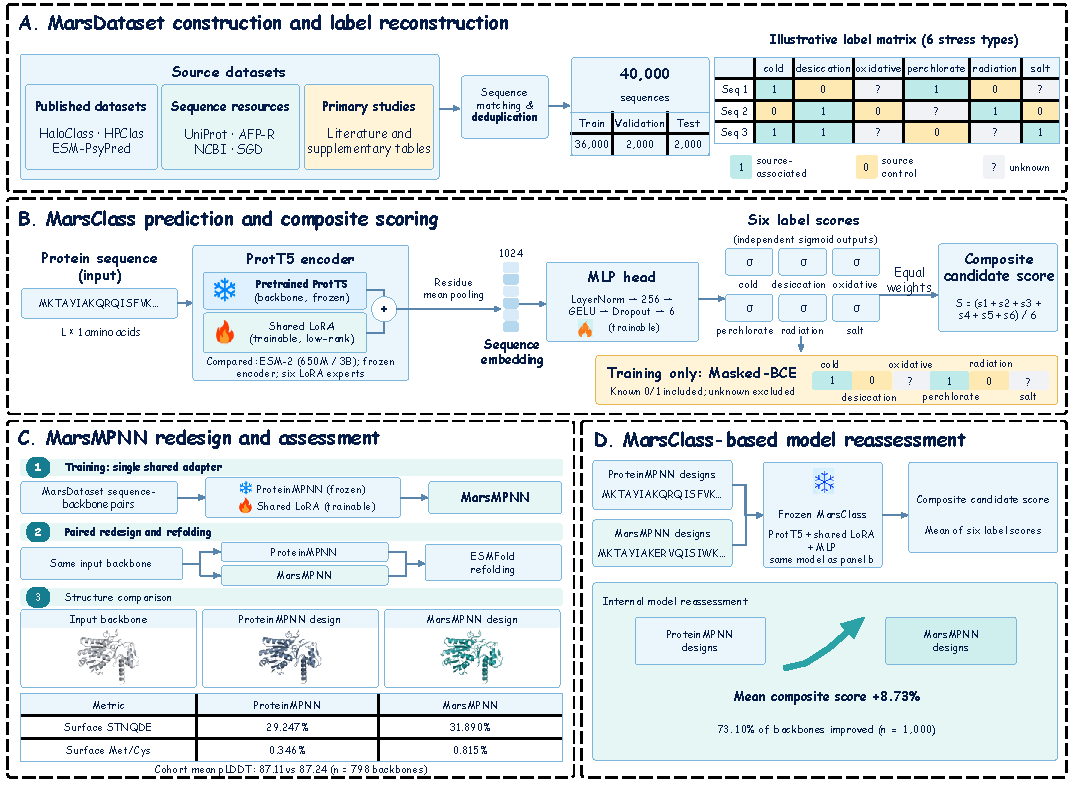
\includegraphics[width=\textwidth]{figures/framework.pdf}
\caption{MarsPro预测、设计与回评框架。MarsDataset支持MarsClass六标签预测和MarsMPNN骨架条件适配。结构分支包含7,979条候选、798个留出骨架和三个匹配生成种子；独立冻结MarsClass回评使用1,000个不同固定测试ID50簇。}
\label{fig:1}
\end{figure*}

\section{相关工作}\label{sec:related}

\subsection{极端环境蛋白资源与预测器}

极端环境研究跨越生物体适应、蛋白生化测量以及适应性蛋白组的序列收集。火星类比与天体生物学研究提供环境背景\cite{ref14,ref15}，CAPP资源则说明宏基因组采样能够形成大规模冷适应蛋白集合\cite{ref31}。不同资源条目的证据含义并不相同：实测酶、家族成员和来自适应性生物的蛋白支持不同强度的结论。MarsDataset保留来源字段用于整理和分层评价；MarsClass仅接收氨基酸序列并预测来源关联归属。

任务特异预测已经从组成特征发展到集成模型和PLM。HPClas使用CatBoost识别嗜盐蛋白\cite{ref18}；HaloClass在生物来源监督下使用PLM表征\cite{ref1}；AHAPC融合手工特征与PLM预测三类极端环境蛋白\cite{ref19}；ESM-PsyPred结合ESM-2嵌入与SVM预测嗜冷蛋白\cite{ref20}。相关研究还涉及嗜冷酶\cite{ref21}、抗氧化蛋白\cite{ref22,ref23}和DNA修复蛋白\cite{ref24}。这些进展支持计算筛选，但独立数据集与不同负例定义阻止了它们被直接拼接为全观测六标签表。

\subsection{蛋白语言模型与参数高效适配}

自监督PLM能够学习包含结构与功能规律的序列表征。ESM在进化序列多样性上扩展无监督学习\cite{ref16}；ProtTrans比较多种Transformer并确立ProtT5的可迁移表征能力\cite{ref2}；Ankh强调蛋白专用架构效率\cite{ref17}。ESMFold进一步表明，PLM表征可以在推理时不执行多序列比对搜索的情况下支持原子级结构预测\cite{ref3}。这些模型构成本文的主干比较，但本文研究的是监督语义与适配策略，而不是提出新的PLM架构。

LoRA冻结预训练权重并学习紧凑的低秩更新\cite{ref4}。本文比较共享六输出适配器与六个任务特异适配器，检验专门化能否带来足以抵消多模型复杂度的预测收益，同时不预设适配器融合一定有效。

\subsection{未知与部分标签学习}

正例与未标注学习明确区分未观测样本与负样本\cite{ref25}。部分标签多标签方法同样将损失限制在具有标注支持的位置，或显式建模标签Mask\cite{ref7}；其他方法还通过随机移除标签处理长尾不均衡\cite{ref26}。MarsPro研究更窄的场景：每个序列与任务位置为正标签、来源对照0或unknown，unknown在损失中的权重为0。

关键不只是减少参与训练的标签，而是保持序列与其来源实际支持条目的对应关系。本文使用未知填0、随机等量Mask、整行打乱Mask及人工移除已知标签进行检验，并始终在相同的已观测验证位置上评价。

\subsection{结构条件蛋白设计与评价}

ProteinMPNN学习骨架条件下的氨基酸分布，相较早期物理方法提高了天然序列恢复率\cite{ref5}。HaloMPNN在嗜盐蛋白组上重新训练逆折叠模型，使生成序列性质向领域分布移动\cite{ref6}。Rosetta可提供互补的建模与能量优化能力\cite{ref27}。这些工作支持领域适配，但组成变化本身不能证明功能。

因此，本文将证据分为序列生成、预测结构置信度、选定溶剂可及表面特征和冻结预测器分数四层。FreeSASA与残基特异最大可及面积用于定义表面特征\cite{ref9,ref10}，US-align用于比较重设计结构与原始输入骨架\cite{ref11}。Pfam、HMMER和MMseqs2支持家族注释与序列关系审计\cite{ref28,ref29,ref30}。分层评价能够暴露单一综合分数会掩盖的权衡。

\FloatBarrier

\section{数据集与标签构建}\label{sec:data}

\subsection{多来源收集与序列关联}

MarsDataset从三条互补路线获得序列。第一条路线是UniProt、NCBI、SGD及专业资源中的稳定标识和注释查询；第二条路线是已发表分类研究的数据和补充材料，包括HaloClass、HPClas及其他任务相关分类集合；第三条路线是原始论文中定义的受测蛋白、家族或蛋白组。序列通过标识与序列内容关联到来源记录，并保留原有证据与标签版本。

同一条蛋白可能出现在多个数据库或论文中。因此，资源数量按唯一序列统计，数据库命中、重复测量和文献端点保留为来源信息，不重复计为独立蛋白。已有去重结果、ID50簇、关系组件、分类群及Pfam侧表用于支持版本连接和评价解释；Pfam、HMMER与MMseqs2分别支持家族注释、谱模型搜索与大规模关系审计\cite{ref28,ref29,ref30}。

\subsection{六任务三态标签}

六类任务为cold、desiccation、oxidative、perchlorate、radiation和salt，分别对应低温、干燥、氧化、高氯酸盐相关、辐射相关及盐适应来源范围。每个序列与任务位置使用1、0或unknown三种状态。1表示符合规定的来源、候选集合或蛋白组归属规则；0表示原数据或补充来源中具有记录依据的对照归属；unknown表示当前证据尚不能确定该任务标签。直接测量、相关机制和来源信息作为不同证据类型保留。

MarsDataset的最终三态标签表保留原始分类器0，只在原unknown位置加入经来源与菌株核对的补充对照0。已有1优先保留，冲突进入独立审计表。新增2,967个0标签位置涉及2,445条唯一序列，另记录883个正标签优先的冲突位置。当前版本不使用抽样伪0。训练时1、原始0和新增来源0权重均为1，unknown权重为0。

\begin{table}[t]
\centering
\caption{数据覆盖：40,000条序列，固定36,000/2,000/2,000划分。}
\label{tab:1}
\footnotesize
\setlength{\tabcolsep}{3pt}
\begin{tabularx}{\columnwidth}{@{}Xrrrrr@{}}
\toprule
任务 & 1 & 0 & Unknown & 验证1/0 & 测试1/0 \\
\midrule
cold & 4,510 & 2,661 & 32,829 & 228/131 & 229/130 \\
desiccation & 7,250 & 1,112 & 31,638 & 366/66 & 360/50 \\
oxidative & 7,175 & 2,458 & 30,367 & 356/129 & 356/124 \\
perchlorate & 2,229 & 262 & 37,509 & 111/14 & 111/11 \\
radiation & 4,583 & 6,812 & 28,605 & 226/339 & 207/364 \\
salt & 8,181 & 3,151 & 28,668 & 406/153 & 412/155 \\
\bottomrule
\end{tabularx}
\end{table}

40,000条序列共对应240,000个标签位置，其中33,928个为1、16,456个为0、189,616个为unknown，未知比例为79.01\%。各任务的分母均为40,000，同一序列可以在多列为1，因此表1各行正标签不能相加作为独立蛋白总数。

\subsection{固定划分与结构子集}

划分前先按50\%序列一致性与80\%双向覆盖度对来源母库进行全局聚类，并在每个连通分量中以与标签无关的规则保留一个代表序列。分类数据采用固定的36,000条训练、2,000条验证和2,000条测试划分，任意两个split之间登记的ID50簇重叠均为0。模型与消融比较使用验证集；最终checkpoint和阈值冻结后，对测试集执行一次性评价。标签重建保留序列的集合归属与ID50标识。

结构数据集包含7,979条来自分类训练集、在v3版本中至少具有一个正标签的序列及其预测结构。ProteinMPNN适配使用6,383条训练、798条验证和798条测试骨架。依据序列标识、完整序列和既有ID50簇检查，结构测试子集与结构训练、验证子集之间未发现重叠。

\section{方法}\label{sec:method}

\subsection{问题定义}

记序列资源为$\mathcal{D}=\{(x_i,\mathbf{y}_i,\mathbf{m}_i)\}_{i=1}^{N}$，其中$x_i$为氨基酸序列，$\mathbf{y}_i\in\{0,1\}^{T}$包含已观测标签的编码值，$\mathbf{m}_i\in\{0,1\}^{T}$指示$T=6$个任务中哪些位置已被观测。$m_{it}=0$表示unknown，而非负例。预测模型估计$\mathbf{p}_i\in[0,1]^T$。设计分支在目标骨架$X$的条件下生成序列$S$，并在登记的同一骨架配对上比较基础模型和适配模型。

\subsection{MarsClass共享蛋白语言模型与六输出分类头}

MarsClass仅接收氨基酸序列。来源标识、物种、属、Pfam及其他溯源字段不进入模型输入，只用于数据整理和分层评价。给定序列x$_i$，蛋白语言模型生成残基级表示H$_i$。对有效残基进行均值池化，排除填充和特殊标记，得到序列表示h$_i$。分类头由层归一化、256维隐藏层、GELU、dropout和六输出线性层组成，最后通过sigmoid分别得到六个标签分数p$_i$$_t$。六个输出独立取值，不要求和为1。

LoRA在选定投影矩阵W$_0$上增加低秩更新，形式为$W=W_0+(\alpha/r)BA$，其中r为低秩维度，A和B为可训练矩阵。主干原始权重保持冻结，适配器和分类头接受下游监督。共享方案以一套适配器服务六任务；六专家方案为各任务分别训练适配器，再将对应输出组成六维预测，或进一步进行固定与动态融合。

\subsection{按任务归一化的Masked-BCE}

记$y_{it}\in\{0,1,?\}$，$m_{it}=\mathbb{1}[y_{it}\ne ?]$。对已观测位置，二元交叉熵为：

\begin{equation}\ell_{it}=-y_{it}\log p_{it}-(1-y_{it})\log(1-p_{it}).\end{equation}

设一个分布式微批中任务t的有效标签数为$n_t=\sum_i m_{it}$，有效任务集合为$\mathcal{T}_B=\{t:n_t>0\}$，则损失为：

\begin{equation}\mathcal{L}_{\mathrm{mask}}=\frac{1}{|\mathcal{T}_B|}\sum_{t\in\mathcal{T}_B}\frac{\sum_i m_{it}\ell_{it}}{n_t}.\end{equation}

该目标先对各任务已观测位置求平均，再对有效任务求平均，使标注数量不同的任务均能贡献训练信号。实现跨设备汇总任务分母，unknown不产生损失。作为对照，普通BCE把unknown编码为0并参与训练。所有模型的验证指标仍在相同的已观测位置上计算，以保持评价目标一致。

\subsection{MarsMPNN联合LoRA重设计}

设计分支以ProteinMPNN的v\_48\_020预训练权重为基础，通过领域LoRA调整给定骨架X时的序列分布p$\theta$(S|X)。采用自回归逆折叠建模，按解码顺序对各位置的氨基酸条件概率进行学习。领域适配将六类来源的数据合并训练，以骨架几何作为条件输入。

联合LoRA生成配置采用r=8、$\alpha$=16及dropout=0.05，适配位置为三个解码层中的W1、W2、W3和输出层W\_out。对798个固定结构测试骨架，普通ProteinMPNN与联合LoRA分别生成三条序列，采样温度0.1。每个骨架和方法均使用匹配的42、43和44号种子，每种方法得到2,394条设计。

六独立LoRA融合是另一条设计方案。该方案先学习六个任务适配器，再比较等权、学习固定权重与动态融合。其训练和结构评价作为独立对照报告。

\subsection{结构与表面特征评价}

全部4,788条设计序列在相同设置下完成再折叠\cite{ref8}。FreeSASA采用Lee--Richards算法、ProtOr半径、1.4 \AA{}探针和20个切片计算溶剂可及表面积\cite{ref9}；残基RSA按Tien等的理论最大ASA归一化\cite{ref10}，以RSA$\geq$0.25定义表面集合。

主要表面特征为STNQDE集合比例和Met/Cys合并比例。各指标先按蛋白计算，再在骨架内对三个种子求均值。设设计与参考在特征k上的取值为$f^{\mathrm{design}}_{ik}$和$f^{\mathrm{ref}}_{ik}$，对应参考绝对距离定义为：

\begin{equation}d_{ik}=\left|f^{\mathrm{design}}_{ik}-f^{\mathrm{ref}}_{ik}\right|,\quad k\in\{\mathrm{STNQDE},\mathrm{MC}\}.\end{equation}

较小的$d_{ik}$表示该特征更接近对应参考。序列回收率与排除亲本后的新颖性分别衡量设计保守性和偏离程度。pLDDT与pTM作为再折叠置信度诊断；US-align将每条设计结构对齐到对应输入骨架，报告对齐RMSD、按参考长度归一化的TM-score和GDT-TS\cite{ref11}。

\subsection{固定测试集重设计与冻结回评}

在固定的2,000条分类测试序列中，于查看预测结果前按SHA256排序选取1,000条至少含一个来源正标签的参考序列。候选须为标准氨基酸、长度不超过500，且各自来自不同的已登记ID50簇。所选参考与MarsClass训练/验证集无精确序列、已登记ID50簇或已登记关系组件重叠，也与现有10,000条ProteinMPNN结构语料无精确序列和已登记ID50簇重叠。ESMFold完成1,000个输入骨架，随后ProteinMPNN与MarsMPNN分别在种子42、43和44上进行匹配设计。

冻结第5轮MarsClass模型，对1,000条参考序列和6,000条设计序列打分，不重新训练，不根据结果重选序列或种子。内部综合评分定义为六个sigmoid输出的等权平均：

\begin{equation}S(x)=\frac{1}{6}\sum_{t=1}^{6}p_t(x),\qquad \Delta S_i=S(x_i^{\mathrm{Mars}})-S(x_i^{\mathrm{base}}).\end{equation}

六个输出以相同权重参与均值。先在每个骨架内平均三个匹配种子，再以1,000个骨架为独立分析单位。比较指标为配对综合分变化、参考序列原有正标签上的得分变化、改善比例，以及六维预测向量到对应参考的欧氏距离。

\section{实验协议}\label{sec:experiments}

评价沿框架中的两组依赖展开。预测实验首先检验证据感知Mask能否改善已观测标签表现，以及单个共享适配器能否保留六个任务专家的精度。设计实验随后测量领域适配如何改变注册骨架对上的表面与结构终点，并检验冻结预测器能否提供一致的事后排序信号。

\subsection{分类比较}

预测实验包含21种主要方法配置和2种补充对照。主比较覆盖ESM-2 650M、ESM-2 3B和ProtT5的冻结主干/LoRA与BCE/Masked-BCE组合，以及ProtT5六专家直接输出、固定融合和动态融合。传统参照包括长度与20种氨基酸组成的独立逻辑回归，以及582维手工特征上的LightGBM和随机森林\cite{ref12,ref13}。丰富特征由长度及其对数、AAC、DPC、CKSAAGP和理化分组比例组成。

深度模型按五轮训练中的验证Macro AP选择checkpoint，F1和MCC所用阈值由验证集确定。Mask对照采用r=8、$\alpha$=16、dropout=0.05、query/value投影、FP16和有效batch 16；任务Mask与随机等量Mask使用相同的42、43、44三个种子。冻结ProtT5设置为五轮、种子42、有效batch 64。三种子Mask对照与主比较分组报告。选定共享ProtT5-LoRA与Masked-BCE后，冻结第5轮checkpoint和六个验证阈值。锁定测试的推理文件仅包含序列标识与序列，六输出概率文件封存哈希后才连接测试标签，此后不再调整模型或阈值。

来源泛化采用四个预注册完整来源折：AAC和ESM-PsyPred低温、AOP2020氧化及HaloClass盐类。每折从训练与验证中移除该来源及其已登记ID50簇和关系组件，共享模型以种子42重新训练五轮并一次性评价已知位置；unknown保持掩蔽，阳性比例作为随机AP参照。

\subsection{预测指标与Mask消融}

分类结果仅在m$_i$$_t$=1的位置上计算。验证集共有2,525个已观测标签位置和9,475个unknown位置；测试集共有2,509个已观测位置，其中1,675个为1、834个为0，另有9,491个unknown位置。unknown不进入评价。AP采用average\_precision\_score，Macro为逐任务平均，Micro将所有已观测位置汇总。报告AP、AUROC、F1、MCC、召回率和校准误差，并同时给出阳性比例以解释不同任务的难度。

随机等量Mask为每个任务随机选取与原Mask相同数量的监督位置；整行打乱Mask保留行模式和各列总量但改变序列对应关系。两者可能把unknown的内部零编码纳入监督，同时移除部分有效标签。人工缺失对照则只在原已知位置中遮蔽25\%的训练标签，验证位置保持不变。上述对照分别检验标签位置匹配与减少已知监督的影响。

\subsection{设计评价与统计分析}

联合LoRA设计包含2,394个同骨架、同种子配对。各指标先在骨架内对42、43和44号种子求均值，再以798个骨架作为独立分析单位。报告配对均值、改善比例、10,000次骨架bootstrap区间，以及经Benjamini--Hochberg校正的Wilcoxon检验。

4,788条设计结构均完成主要终点评价，形成2,394个完整配对，没有失败或主要指标缺失。

\subsection{固定测试回评统计}

回评保留全部1,000个参考骨架及其三种子配对设计。推理采用冻结的第5轮checkpoint；哨兵样本的最大绝对误差为0。先在骨架内对三个匹配种子求均值，再以骨架为单位进行10,000次配对bootstrap和双侧符号检验。逐任务统计仅使用参考序列在该任务上标为1的骨架，不将unknown当作负例。

\section{结果}\label{sec:results}

\subsection{缺失标签感知学习改善预测表现}

表2是统一协议下的编码器选择对照：所有神经网络行使用相同数据划分、标签语义和评价位置，只改变PLM主干、参数适配方式和监督规则。共享ProtT5-LoRA结合Masked-BCE取得该组比较中最高的验证Macro AP 0.9771，AUROC、F1和MCC分别为0.9623、0.9328和0.7934。图2分别展示Mask、LoRA、随机种子及专家融合的影响。

模型选择冻结后，共享模型在一次性锁定测试上取得0.97529的Macro AP、0.96003的Macro AUROC、0.91756的Macro F1和0.74118的Macro MCC，Micro AP为0.98210。相较验证集，Macro AP变化为$-0.00180$；F1和MCC分别下降0.01522和0.05225，说明排序性能稳定，但固定阈值下存在一定跨划分漂移。六任务测试AP依次为cold 0.96958、desiccation 0.99552、oxidative 0.98162、perchlorate 0.99937、radiation 0.92124和salt 0.98439。高氯酸盐测试已知负例仅11条，因此其近满分结果需结合分母解释。

\subsection{完整来源泛化}

四个已知标签挑战分别包含1,392条AAC低温、1,924条ESM-PsyPred低温、1,566条AOP2020氧化和4,095条HaloClass盐类序列。AP/阳性比例依次为0.327/0.175、0.198/0.161、0.226/0.108和0.903/0.437，AUROC为0.691、0.657、0.736和0.946。四折排序均高于随机，但验证阈值下的负例召回为0.047至0.741，MCC为0.063至0.234。因此，完整来源重训练支持跨来源排序，但不能给出来源不变的统一阈值。

\begin{table*}[t]
\centering
\caption{已观测验证标签上的编码器、适配方式与监督策略对照；各指标最优值加粗。}
\label{tab:2}
\footnotesize
\setlength{\tabcolsep}{3pt}
\begin{tabularx}{\textwidth}{@{}Xllrrrr@{}}
\toprule
主干/特征 & 适配 & 监督 & AP & AUROC & F1 & MCC \\
\midrule
\textbf{ProtT5} & \textbf{LoRA} & \textbf{Masked-BCE} & \textbf{0.9771} & \textbf{0.9623} & \textbf{0.9328} & \textbf{0.7934} \\
ProtT5 & LoRA & BCE & 0.9539 & 0.9083 & 0.8674 & 0.6204 \\
ProtT5 & 冻结 & Masked-BCE & 0.9741 & 0.9570 & 0.9275 & 0.7882 \\
ProtT5 & 冻结 & BCE & 0.9507 & 0.8979 & 0.8652 & 0.6084 \\
\midrule
ESM-2 3B & LoRA & Masked-BCE & 0.9749 & 0.9570 & 0.9298 & 0.7931 \\
ESM-2 3B & LoRA & BCE & 0.9509 & 0.8936 & 0.8611 & 0.5867 \\
ESM-2 3B & 冻结 & Masked-BCE & 0.9734 & 0.9548 & 0.9258 & 0.7681 \\
ESM-2 3B & 冻结 & BCE & 0.9468 & 0.8899 & 0.8592 & 0.5842 \\
\midrule
ESM-2 650M & LoRA & Masked-BCE & 0.9725 & 0.9550 & 0.9217 & 0.7588 \\
ESM-2 650M & LoRA & BCE & 0.9461 & 0.8868 & 0.8562 & 0.5735 \\
ESM-2 650M & 冻结 & Masked-BCE & 0.9702 & 0.9507 & 0.9220 & 0.7553 \\
ESM-2 650M & 冻结 & BCE & 0.9430 & 0.8803 & 0.8537 & 0.5696 \\
\midrule
丰富手工特征 & LightGBM & 已知标签 & 0.9353 & 0.8856 & 0.8757 & 0.5968 \\
丰富手工特征 & RF & 已知标签 & 0.9189 & 0.8424 & 0.8349 & 0.4959 \\
长度+AAC & LR & 已知标签 & 0.8970 & 0.8179 & 0.8095 & 0.4694 \\
\bottomrule
\end{tabularx}
\end{table*}

\begin{figure*}[!t]
\centering
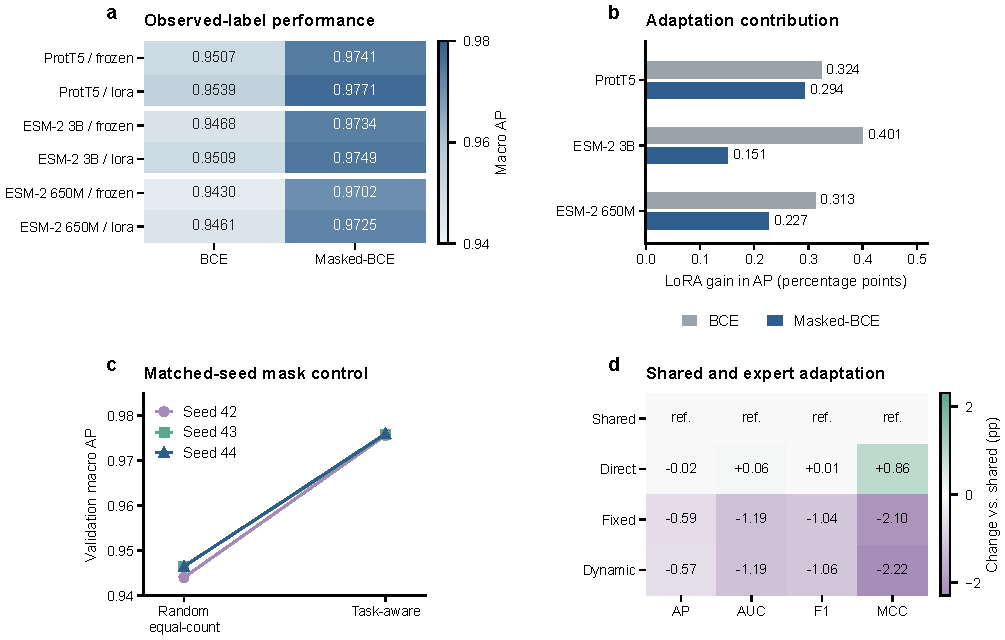
\includegraphics[width=\textwidth]{figures/ablation.pdf}
\caption{已观测验证标签上的预测消融。a：不同主干、适配与损失的Macro AP热图；b：LoRA相对冻结编码器的AP增量，单位为百分点；c：独立Mask对照中42至44三个匹配种子；d：专家相对共享模型的指标差值，单位为百分点，共享行为参照。a、b及d报告单次运行比较。}
\label{fig:2}
\end{figure*}

LoRA在三种主干上均带来进一步的AP提升。在Masked-BCE设置下，ProtT5由冻结主干的0.97415提高至0.97709，增量为0.00294；ESM-2 650M和3B分别提高0.00227和0.00151，对应0.227和0.151个百分点。三种主干的AUROC也均随LoRA适配提高。这些结果表明，在保留预训练表征的基础上，低秩适配能够进一步学习六任务所需的序列信息。

Masked-BCE在冻结及LoRA设置下均提高预测表现。对共享ProtT5-LoRA，使用Masked-BCE相较于未知填0的BCE，AP提高0.02315，MCC提高0.17304；冻结ProtT5的AP由0.95070提高至0.97415。ESM-2 650M冻结、650M LoRA、3B冻结及3B LoRA的AP分别提高0.02717、0.02631、0.02654和0.02404。因此，缺失标签处理和LoRA适配分别在监督目标与模型参数两个层面发挥作用，共同构成本文的预测方法。

\subsection{共享适配达到与复杂专家系统相近的表现}

六专家直接输出的Macro AP为0.97686，与共享LoRA的0.97709相差0.00023；其AUROC、F1和MCC分别略高于共享方案。固定与动态融合的AP则分别为0.97116和0.97138，未超过专家直接输出。类别平衡与训练子集对照的AP同样低于共享方案。共享方案以单套适配器获得接近独立专家的表现，因此被采用为框架的主要预测入口。

\begin{table*}[t]
\centering
\caption{ProtT5消融。下半部分为独立Mask对照批次，多种子指标报告均值，AP标准差为样本标准差。}
\label{tab:3}
\footnotesize
\setlength{\tabcolsep}{3pt}
\begin{tabularx}{\textwidth}{@{}Xrrrrrr@{}}
\toprule
设置 & 运行数 & AP & AUROC & F1 & MCC & AP标准差 \\
\midrule
共享LoRA & 1 & 0.97709 & 0.96227 & 0.93278 & 0.79342 & -- \\
六专家直接输出 & 1 & 0.97686 & 0.96286 & 0.93285 & 0.80207 & -- \\
六专家固定融合 & 1 & 0.97116 & 0.95032 & 0.92237 & 0.77244 & -- \\
六专家动态融合 & 1 & 0.97138 & 0.95033 & 0.92215 & 0.77125 & -- \\
类别平衡损失 & 1 & 0.97636 & 0.95927 & 0.93030 & 0.78111 & -- \\
内部训练子集 & 1 & 0.97473 & 0.95867 & 0.92483 & 0.78753 & -- \\
\midrule
任务感知Mask & 3 & 0.97579 & 0.95917 & 0.92889 & 0.78423 & 0.00017 \\
随机等量Mask & 3 & 0.94567 & 0.88668 & 0.85101 & 0.58332 & 0.00143 \\
整行打乱Mask & 1 & 0.94088 & 0.87504 & 0.82214 & 0.54072 & -- \\
已知标签遮蔽25\% & 1 & 0.97504 & 0.95665 & 0.92808 & 0.77836 & -- \\
\bottomrule
\end{tabularx}
\end{table*}

\subsection{Mask对照区分标签语义与标签数量}

独立三种子实验中，任务感知Mask的Macro AP为0.97579$\pm$0.00017，随机等量Mask为0.94567$\pm$0.00143，配对种子的方向一致，均值差为0.03012。整行打乱Mask降至0.94088。仅在已知位置人工遮蔽25\%标签的结果为0.97504，在该单次运行中接近完整任务Mask。

表3汇总Mask对照结果，图2c展示相同种子的配对比较。

丰富手工特征上的LightGBM优于长度与AAC逻辑回归，任务感知PLM三种子均值进一步高出LightGBM 0.04049 AP。该结果表明，预训练序列表征结合低秩适配与任务感知监督，能够在所比较的手工特征之外提供额外预测信息。

\subsection{逐任务支持规模与校准}

共享ProtT5-LoRA在辐射相关任务上的AP为0.9275，低于其余五类；高氯酸盐相关任务达到0.9991，其已观测验证位置为125个，其中0标签14个。表1列出各任务验证支持数，完整逐任务指标与校准数值保存在附带数据中。

ECE采用10分箱。共享模型Micro AP为0.98175。已观测位置的Macro和Micro阳性比例分别为0.70511和0.67050，为解释AP提供相应的标签比例参照。

\subsection{匹配种子领域适配改变表面组成}

联合LoRA设计评价包含798个唯一骨架和三个匹配种子。设计表面STNQDE比例由29.25\%提高至31.89\%，其到配对参考的绝对距离由0.11192降至0.09327，相对下降16.67\%。2,394个设计配对中62.16\%改善，骨架级均值差为-0.01865，95\%置信区间为[-0.02275, -0.01468]。

表面Met/Cys比例由0.346\%提高至0.815\%，到参考的绝对距离由0.02504降至0.02071，相对下降17.30\%。71.89\%的设计配对改善，骨架级均值差为-0.00433，95\%置信区间为[-0.00468, -0.00399]。

序列回收率由37.91\%提高至41.24\%，增加3.33个百分点，95\%置信区间为[3.06, 3.62]；排除亲本后的新颖性没有明确变化。以上结果表明，领域LoRA调整了骨架条件生成分布，使设计序列在选定表面组成上更接近对应参考。

\begin{figure*}[!t]
\centering
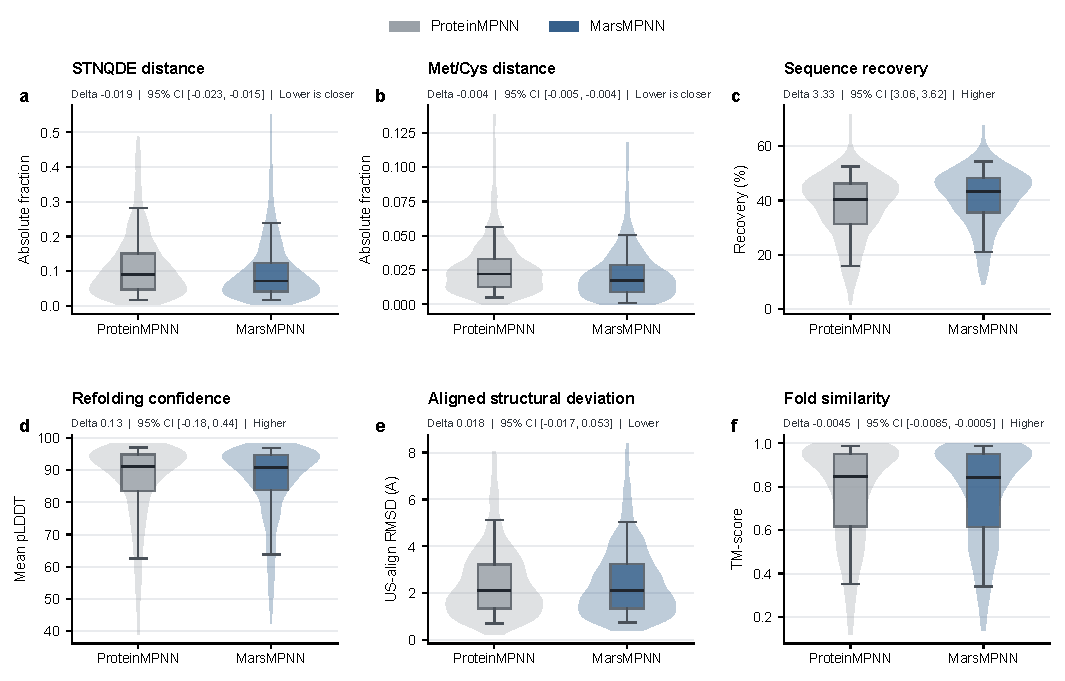
\includegraphics[width=\textwidth]{figures/design.pdf}
\caption{798个登记骨架和2,394个匹配种子设计配对的评价。每个分布包含每骨架三个种子的均值。a、b：表面STNQDE和Met/Cys到对应参考的绝对距离。c：序列回收率。d：平均pLDDT。e、f：US-align RMSD及按参考长度归一化的TM-score。小提琴表示密度，盒体表示四分位距与中位数，须线为第5至95百分位。图内给出MarsMPNN减ProteinMPNN的均值差和95\%骨架bootstrap区间。}
\label{fig:3}
\end{figure*}

\subsection{结构保持与内部预测一致性}

普通ProteinMPNN与MarsMPNN的平均pLDDT分别为87.11和87.24，差值+0.13，95\%置信区间为[-0.18, 0.44]。US-align RMSD由2.426变为2.444 \AA{}，差值+0.018 \AA{}，95\%置信区间为[-0.017, 0.053]。

按参考长度归一化的TM-score由0.7700降至0.7655，差值为-0.0045，95\%置信区间为[-0.0085, -0.0005]；GDT-TS下降0.764个百分点。领域适配在保持近似再折叠置信度的同时改变表面组成和序列回收率，但没有改善结构保真度。在这798条MarsClass训练已见参考上，内部六输出均分由0.6266升至0.6687，随后使用独立固定测试参考执行更严格回评。

\subsection{固定测试集回评提供一致的排序信号}

相较ProteinMPNN，MarsMPNN的骨架均值六输出综合分由0.61854提高至0.67251，相对提升8.73\%。配对均值差为+0.05397，95\%区间为[0.04889, 0.05925]，双侧符号检验\(p=6.25\times10^{-50}\)。1,000个骨架中731个改善，占73.10\%。仅在每条参考序列原有正标签上汇总时，均分由0.65359提高至0.74563，差值为+0.09203，95\%区间为[0.07757, 0.10656]，660/1,000个骨架改善。

\begin{figure*}[!t]
\centering
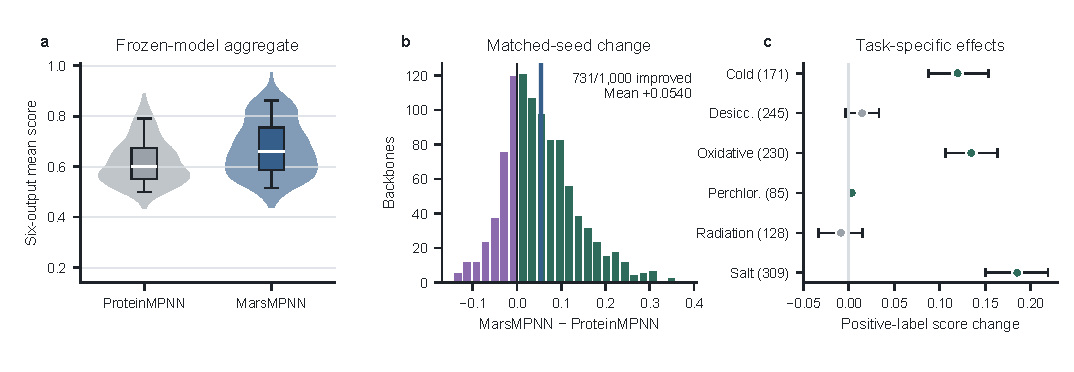
\includegraphics[width=\textwidth]{figures/rescoring.pdf}
\caption{冻结MarsClass在1,000条预测盲选、且各自来自不同已登记ID50簇的固定测试参考上的回评。a：平均三个匹配种子后的骨架级六输出综合分布；b：MarsMPNN减ProteinMPNN的配对变化分布，竖线和色带分别表示均值和95\%配对bootstrap区间；c：各参考正标签任务上的均值变化及95\%配对bootstrap区间。}
\label{fig:4}
\end{figure*}

六维预测到对应参考向量的平均距离由0.98189降至0.83931，700/1,000个骨架更加接近参考。逐任务正标签变化分别为：低温+0.1196、干燥+0.0145、氧化+0.1349、高氯酸盐+0.0033、辐射-0.0087和盐适应+0.1853。低温、氧化和盐适应的区间明确高于0；高氯酸盐变化很小且分数接近饱和；干燥和辐射的区间跨0。因此，综合分移动在匹配种子上可重复，但并非六个任务均匀提升。

\section{讨论}\label{sec:discussion}

MarsPro的核心结果是，显式标签语义与生成目标同样重要。MarsClass的Masked-BCE在ProtT5和两种规模ESM-2上均带来一致收益，包括冻结编码器。随机等量Mask和整行打乱Mask将该收益归因于正确的序列与任务对应关系，而不是监督位置减少。六个任务适配器接近共享模型，但融合没有提高AP。锁定测试保持资源内部排序，完整来源重训练则在高于阳性比例的同时揭示来源依赖的阈值迁移。

共享适配与任务特异适配的比较澄清了模型复杂度的作用。六个独立专家接近共享模型，但固定融合和动态融合没有提高AP。对当前资源而言，跨任务参数共享是更经济的配置。任务特异监督更密集时，专门化是否有益仍需独立数据检验。

设计分支回答了不同问题。领域适配ProteinMPNN把HaloMPNN在单一嗜盐领域的重训练逻辑\cite{ref6}扩展到多来源资源。三个匹配种子显示，STNQDE和Met/Cys到对应参考的距离均下降，序列回收率提高。US-align RMSD和pLDDT相近，但TM-score与GDT-TS略低，因此结果应解释为序列与表面组成的选择性移动，而不是结构保真度改善。

冻结MarsClass回评连接了预测与设计分支。在MarsClass训练/验证未见的固定测试亲本簇上，平均六输出综合分提高8.73\%，731/1,000个骨架改善。这说明MarsMPNN产生的序列更接近固定预测器在相关来源上学到的模式。相比训练集回评，这一设计提高了独立性；但评价仍由MarsClass给出，因此是模型介导的一致性证据，而不是功能验证。

综合来看，工作流将来源证据、预测监督、序列生成、结构分析和事后评分作为不同阶段。实际输出是一组带有来源、模型与证据边界的候选排序。其活性、稳定性、溶解性和火星类比表型仍需独立数据、关系隔离评价和实验测试。

\section{局限性}

本研究标签描述来源、家族或蛋白组归属，而不是每条蛋白经过实验确认的耐受功能。四个单种子来源折只覆盖低温、氧化和盐类，不等同于分类群、家族或全局关系组件留出。对照不均衡、组成捷径和来源依赖阈值仍影响部署；随机及打乱Mask同时改变监督位置和零编码噪声，现有多种子结果也不能代表完整的来源泛化不确定性。

匹配种子结构研究的798条参考与固定测试回评的1,000条参考回答不同问题。前者均进入过MarsClass训练集；后者与MarsClass训练/验证集无精确序列、已登记ID50簇和已登记关系组件重叠。6,000条回评设计序列与训练/验证集无精确匹配，但尚未对全部设计序列与完整训练集重做ID50聚类。事后等权平均不是经校准的多胁迫耐受概率；高氯酸盐输出接近饱和，辐射和干燥的区间跨0，都限制了综合提升的功能解释。

表面特征变化证明的是对指定参考分布的接近，而非实测溶解度、干燥保护或抗氧化能力。三个匹配种子降低了采样不确定性，但TM-score与GDT-TS的小幅下降说明领域适配没有改善折叠保持。更广泛的来源折、ID30、家族或分类群留出评价、独立评价器和湿实验，将分别检验远同源泛化、模型自洽偏差与目标表型。

\section{结论}\label{sec:conclusion}

MarsPro在MarsDataset多来源标注、MarsClass预测和MarsMPNN逆折叠评估之间保持证据状态。MarsClass达到0.9771的验证Macro AP和0.9753的锁定测试Macro AP，四个来源折均高于阳性比例。在798个骨架和三个匹配种子上，MarsMPNN设计使STNQDE与Met/Cys表面参考距离分别下降16.67\%和17.30\%，并保持相近的pLDDT与US-align RMSD。在1,000个固定测试ID50簇上，冻结MarsClass回评综合分提高8.73\%，73.10\%的骨架级比较改善。数据资源、掩码目标、严格测试和注册设计分析共同形成可复现的实验候选优选依据。

\section*{AI辅助声明}

OpenAI Codex用于辅助结构整理与数值检查；作者核验了全部证据与结论。

\FloatBarrier

\begin{thebibliography}{32}
\bibitem{ref14} R. Cavicchioli, ``Extremophiles and the search for extraterrestrial life,'' \textit{Astrobiology}, vol. 2, no. 3, pp. 281--292, Aug. 2002, doi: \href{https://doi.org/10.1089/153110702762027862}{\nolinkurl{10.1089/153110702762027862}}.

\bibitem{ref15} A. G. Fair\'en \textit{et al.}, ``Astrobiology through the ages of Mars: The study of terrestrial analogues to understand the habitability of Mars,'' \textit{Astrobiology}, vol. 10, no. 8, pp. 821--843, Oct. 2010, doi: \href{https://doi.org/10.1089/ast.2009.0440}{\nolinkurl{10.1089/ast.2009.0440}}.

\bibitem{ref31} G. Varliero \textit{et al.}, ``Microbial characterisation and Cold-Adapted Predicted Protein database construction from the active layer of Greenland's permafrost,'' \textit{FEMS Microbiol. Ecol.}, vol. 97, no. 10, Art. no. fiab127, Oct. 2021, doi: \href{https://doi.org/10.1093/femsec/fiab127}{\nolinkurl{10.1093/femsec/fiab127}}.

\bibitem{ref32} K. S. Siddiqui and R. Cavicchioli, ``Cold-adapted enzymes,'' \textit{Annu. Rev. Biochem.}, vol. 75, no. 1, pp. 403--433, Jun. 2006, doi: \href{https://doi.org/10.1146/annurev.biochem.75.103004.142723}{\nolinkurl{10.1146/annurev.biochem.75.103004.142723}}.

\bibitem{ref16} A. Rives \textit{et al.}, ``Biological structure and function emerge from scaling unsupervised learning to 250 million protein sequences,'' \textit{Proc. Natl. Acad. Sci. USA}, vol. 118, no. 15, Art. no. e2016239118, Apr. 2021, doi: \href{https://doi.org/10.1073/pnas.2016239118}{\nolinkurl{10.1073/pnas.2016239118}}.

\bibitem{ref2} A. Elnaggar \textit{et al.}, ``ProtTrans: Toward understanding the language of life through self-supervised learning,'' \textit{IEEE Trans. Pattern Anal. Mach. Intell.}, vol. 44, no. 10, pp. 7112--7127, Oct. 2022, doi: \href{https://doi.org/10.1109/TPAMI.2021.3095381}{\nolinkurl{10.1109/TPAMI.2021.3095381}}.

\bibitem{ref17} A. Elnaggar \textit{et al.}, ``Ankh: Optimized protein language model unlocks general-purpose modelling,'' \textit{arXiv preprint arXiv:2301.06568}, Jan. 2023, doi: \href{https://doi.org/10.48550/arXiv.2301.06568}{\nolinkurl{10.48550/arXiv.2301.06568}}.

\bibitem{ref1} K. Narang, A. Nath, W. Hemstrom, and S. K. S. Chu, ``HaloClass: Salt-tolerant protein classification with protein language models,'' \textit{Protein J.}, vol. 43, no. 6, pp. 1035--1044, Dec. 2024, doi: \href{https://doi.org/10.1007/s10930-024-10236-7}{\nolinkurl{10.1007/s10930-024-10236-7}}.

\bibitem{ref18} S. Hu \textit{et al.}, ``HPClas: A data-driven approach for identifying halophilic proteins based on CatBoost,'' \textit{mLife}, vol. 3, no. 4, pp. 515--526, Dec. 2024, doi: \href{https://doi.org/10.1002/mlf2.12125}{\nolinkurl{10.1002/mlf2.12125}}.

\bibitem{ref20} C. Peng \textit{et al.}, ``ESM-PsyPred: Leveraging protein language models for accurate prediction of psychrophilic proteins,'' \textit{Interdiscip. Sci.}, early access, Jan. 29, 2026, doi: \href{https://doi.org/10.1007/s12539-025-00810-7}{\nolinkurl{10.1007/s12539-025-00810-7}}.

\bibitem{ref21} A. Huang, F. Lu, and F. Liu, ``Discrimination of psychrophilic enzymes using machine learning algorithms with amino acid composition descriptor,'' \textit{Front. Microbiol.}, vol. 14, Art. no. 1130594, Feb. 2023, doi: \href{https://doi.org/10.3389/fmicb.2023.1130594}{\nolinkurl{10.3389/fmicb.2023.1130594}}.

\bibitem{ref19} M. Lu and T. Liu, ``AHAPC: Multi-source feature fusion and ensemble learning for multiclass extremophilic protein prediction,'' \textit{Anal. Biochem.}, vol. 709, Art. no. 116005, Feb. 2026, doi: \href{https://doi.org/10.1016/j.ab.2025.116005}{\nolinkurl{10.1016/j.ab.2025.116005}}.

\bibitem{ref22} L. H. T. Lam \textit{et al.}, ``Machine learning model for identifying antioxidant proteins using features calculated from primary sequences,'' \textit{Biology}, vol. 9, no. 10, Art. no. 325, Oct. 2020, doi: \href{https://doi.org/10.3390/biology9100325}{\nolinkurl{10.3390/biology9100325}}.

\bibitem{ref23} G. Rukh, S. Akbar, G. Rehman, F. K. Alarfaj, and Q. Zou, ``StackedEnC-AOP: Prediction of antioxidant proteins using transform evolutionary and sequential features based multi-scale vector with stacked ensemble learning,'' \textit{BMC Bioinformatics}, vol. 25, no. 1, Art. no. 256, Aug. 2024, doi: \href{https://doi.org/10.1186/s12859-024-05884-6}{\nolinkurl{10.1186/s12859-024-05884-6}}.

\bibitem{ref24} J. B. Brown and T. Akutsu, ``Identification of novel DNA repair proteins via primary sequence, secondary structure, and homology,'' \textit{BMC Bioinformatics}, vol. 10, no. 1, Art. no. 25, Jan. 2009, doi: \href{https://doi.org/10.1186/1471-2105-10-25}{\nolinkurl{10.1186/1471-2105-10-25}}.

\bibitem{ref3} Z. Lin \textit{et al.}, ``Evolutionary-scale prediction of atomic-level protein structure with a language model,'' \textit{Science}, vol. 379, no. 6637, pp. 1123--1130, Mar. 2023, doi: \href{https://doi.org/10.1126/science.ade2574}{\nolinkurl{10.1126/science.ade2574}}.

\bibitem{ref4} E. J. Hu \textit{et al.}, ``LoRA: Low-rank adaptation of large language models,'' in \textit{Proc. Int. Conf. Learn. Represent. (ICLR)}, 2022. [Online]. Available: \url{https://openreview.net/forum?id=nZeVKeeFYf9}

\bibitem{ref25} J. Bekker and J. Davis, ``Learning from positive and unlabeled data: A survey,'' \textit{Mach. Learn.}, vol. 109, no. 4, pp. 719--760, Apr. 2020, doi: \href{https://doi.org/10.1007/s10994-020-05877-5}{\nolinkurl{10.1007/s10994-020-05877-5}}.

\bibitem{ref7} T. Durand, N. Mehrasa, and G. Mori, ``Learning a deep ConvNet for multi-label classification with partial labels,'' in \textit{Proc. IEEE/CVF Conf. Comput. Vis. Pattern Recognit. (CVPR)}, Long Beach, CA, USA, Jun. 2019, pp. 647--657, doi: \href{https://doi.org/10.1109/CVPR.2019.00074}{\nolinkurl{10.1109/CVPR.2019.00074}}.

\bibitem{ref26} K. Duarte, Y. Rawat, and M. Shah, ``PLM: Partial label masking for imbalanced multi-label classification,'' in \textit{Proc. IEEE/CVF Conf. Comput. Vis. Pattern Recognit. Workshops (CVPRW)}, Jun. 2021, pp. 2733--2742, doi: \href{https://doi.org/10.1109/CVPRW53098.2021.00308}{\nolinkurl{10.1109/CVPRW53098.2021.00308}}.

\bibitem{ref5} J. Dauparas \textit{et al.}, ``Robust deep learning-based protein sequence design using ProteinMPNN,'' \textit{Science}, vol. 378, no. 6615, pp. 49--56, Oct. 2022, doi: \href{https://doi.org/10.1126/science.add2187}{\nolinkurl{10.1126/science.add2187}}.

\bibitem{ref6} A. L. Lee, A. Seamann, G. Chung, C. Zhao, R. Maddamsetti, and S. D. Khare, ``HaloMPNN: Retraining ProteinMPNN on halophilic proteomes for salt-tolerant enzyme design,'' \textit{bioRxiv}, preprint 2026.08.02.742362, Aug. 4, 2026, doi: \href{https://doi.org/10.64898/2026.08.02.742362}{\nolinkurl{10.64898/2026.08.02.742362}}.

\bibitem{ref27} J. K. Leman \textit{et al.}, ``Macromolecular modeling and design in Rosetta: Recent methods and frameworks,'' \textit{Nat. Methods}, vol. 17, no. 7, pp. 665--680, Jul. 2020, doi: \href{https://doi.org/10.1038/s41592-020-0848-2}{\nolinkurl{10.1038/s41592-020-0848-2}}.

\bibitem{ref9} S. Mitternacht, ``FreeSASA: An open source C library for solvent accessible surface area calculations,'' \textit{F1000Research}, vol. 5, Art. no. 189, Feb. 2016, doi: \href{https://doi.org/10.12688/f1000research.7931.1}{\nolinkurl{10.12688/f1000research.7931.1}}.

\bibitem{ref10} M. Z. Tien, A. G. Meyer, D. K. Sydykova, S. J. Spielman, and C. O. Wilke, ``Maximum allowed solvent accessibilities of residues in proteins,'' \textit{PLoS ONE}, vol. 8, no. 11, Art. no. e80635, Nov. 2013, doi: \href{https://doi.org/10.1371/journal.pone.0080635}{\nolinkurl{10.1371/journal.pone.0080635}}.

\bibitem{ref11} C. Zhang, M. Shine, A. M. Pyle, and Y. Zhang, ``US-align: Universal structure alignments of proteins, nucleic acids, and macromolecular complexes,'' \textit{Nat. Methods}, vol. 19, no. 9, pp. 1109--1115, Sep. 2022, doi: \href{https://doi.org/10.1038/s41592-022-01585-1}{\nolinkurl{10.1038/s41592-022-01585-1}}.

\bibitem{ref28} S. El-Gebali \textit{et al.}, ``The Pfam protein families database in 2019,'' \textit{Nucleic Acids Res.}, vol. 47, no. D1, pp. D427--D432, Jan. 2019, doi: \href{https://doi.org/10.1093/nar/gky995}{\nolinkurl{10.1093/nar/gky995}}.

\bibitem{ref29} S. R. Eddy, ``Accelerated profile HMM searches,'' \textit{PLoS Comput. Biol.}, vol. 7, no. 10, Art. no. e1002195, Oct. 2011, doi: \href{https://doi.org/10.1371/journal.pcbi.1002195}{\nolinkurl{10.1371/journal.pcbi.1002195}}.

\bibitem{ref30} M. Steinegger and J. S\"oding, ``MMseqs2 enables sensitive protein sequence searching for the analysis of massive data sets,'' \textit{Nat. Biotechnol.}, vol. 35, no. 11, pp. 1026--1028, Nov. 2017, doi: \href{https://doi.org/10.1038/nbt.3988}{\nolinkurl{10.1038/nbt.3988}}.

\bibitem{ref8} S. Candido \textit{et al.}, ``Language modeling materializes a world model of protein biology,'' \textit{bioRxiv}, preprint 2026.06.03.729735, Jun. 4, 2026, doi: \href{https://doi.org/10.64898/2026.06.03.729735}{\nolinkurl{10.64898/2026.06.03.729735}}.

\bibitem{ref12} G. Ke \textit{et al.}, ``LightGBM: A highly efficient gradient boosting decision tree,'' in \textit{Adv. Neural Inf. Process. Syst.}, vol. 30, 2017, pp. 3146--3154.

\bibitem{ref13} L. Breiman, ``Random forests,'' \textit{Mach. Learn.}, vol. 45, no. 1, pp. 5--32, Oct. 2001, doi: \href{https://doi.org/10.1023/A:1010933404324}{\nolinkurl{10.1023/A:1010933404324}}.
\end{thebibliography}
\end{document}
